% !TEX root=./report.tex

\section{Approach}
In this paper we propose two algorithms to solve distinct problems that arise from the real-world disturbances that act upon the \ITS{}.

\subsection{Dynamic stabilization}
\label{sec:dynamic_stabilization}
The gantry bridges to which the cameras are mounted are prone to environmental influences. 
These influences include, but not exclusively, wind and vibrations from passing vehicles.
These external influences bring the cameras into a swinging state which introduces jittery motion in the video feeds.

Although the displacements of the camera only span a small range around its resting position, the influences in on the images amplify by the huge distances the cameras overview.

To mitigate the noise added by the jittery motion we propose the pipeline displayed in \autoref{fig:dynamic_stabilization_algorithm}.

\begin{figure}[t]
  \begin{center}
  % \fbox{\rule{0pt}{2in} \rule{0.9\linewidth}{0pt}}
     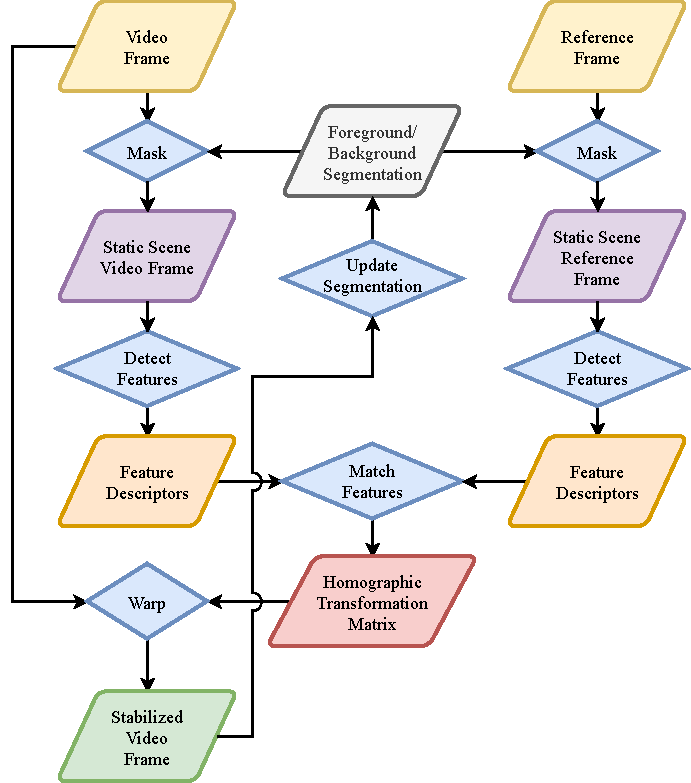
\includegraphics[width=0.8\linewidth]{diagrams/DynamicStabilization.pdf}
  \end{center}
     \caption{}
  \label{fig:dynamic_stabilization_algorithm}
  \end{figure}

% \paragraph{Frame retrieval}
% The first step in the algorithm is to retrieve the current frame from the camera.

\paragraph{Removing dynamic foreground scene}
We only want to find features on the non-moving \Sc{} objects, \eg{} the road, poles, guardrails and bridges. 
As these features are expected to not move between frames, aligning these during image warping ensures that the scene stays static.
Moving vehicles are thus excluded from the detection and do not contribute in the algorithm.

Hence, we mask the current video frame and the stable reference frame using a background segmentation based on
the \emph{Improved Adaptive Gaussian Mixture Model for Background Subtraction} proposed by Zoran Zivkovic \etal{} \cite{zivkovic10.5555/1018428.1020644,zivkovic10.1016/j.patrec.2005.11.005,opencv_library}.

Additionally it speeds up the algorithm. 

Maybe append more about warmup for MOG2.

\paragraph{Feature detection}
We are looking for specific patterns or specific features which are unique, can be easily tracked and can be easily compared. (Taken from OpenCV)

Hence, on the \Sc{} of the video frame and reference frame we perform feature
detection to retrieve the descriptors and pixel locations of prominent image
parts.

There exists many different implementations of feature detectors and descriptors
as described by Kumar \etal{} \cite{kumar2014survey}. We mainly focus on the
implementations of SIFT \cite{lowe10.1023/B:VISI.0000029664.99615.94}, SURF
\cite{bay10.1007/11744023_32} and ORB \cite{rublee6126544} feature detectors and
descriptors, Fast \cite{Ghahremani_2021} feature detector with FREAK \cite{alahi6247715} feature
descriptors and Star \cite{agrawal2008censure} feature detector with BRIEF \cite{calonder10.5555/1888089.1888148} feature descriptors coming from the OpenCV library \cite{opencv_library}. 

\paragraph{Feature matching}
Feature matching compares the features of one frame to the features of the other frame.
A match is reported if the feature descriptors of two compared features surpass a specific dynamic
threshold \cite{lowe10.1023/B:VISI.0000029664.99615.94} regarding some feature
dependent metric \cite{kumar2014survey}.
These feature matches establish a spatial relationship in pixel space between
the two frames.

Based on this spatial pixel relationship we can now compute the homographic
transformation between the two frames. The transformation describes a
perspective transformation $H$ between $(x'_i, y'_i, 1)^T$ and
$(x_i, y_i, 1)^T$ so that
\begin{equation}
 s_i  * (x'_i, y'_i, 1)^T \sim H * (x_i, y_i, 1)^T
\end{equation}
and minimizes the back-projection error.

The implementation is included in the OpenCV library \cite{opencv_library}.

\paragraph{Image alignment}
With the given homographic transformation the current video frame is now warped so that the matches align in pixel space.
As a consequence the static scene is now aligned perfectly between the two frames. 
As the keyframe is stable and does not change over time the current video frame
is now also stabilized as the motion of the static scene is minimized.

\paragraph{Foreground/Background segmentation upate}
As a last step the foreground/background segmentation is updated using the new
stabilized frame. This ensures that for the next frame the segmentation
distinguishes the static scene and dynamic foreground. 

This reduces the search space for the feature detectors and prohibits matches
between static scene and dynamic foreground objects. Hence, the algorithm is
robustified and speed up.
